\section{Appendix}
\section*{Reading Guide}\label{sec:reading_guide}
\begin{center}\small
\begin{tikzpicture}
    [auto,
     decision/.style={diamond, draw=blue, thick, fill=blue!10,
                      text width=4.5em,align=flush center,
                      inner sep=1pt},
    block/.style ={rectangle, draw=blue, thick, fill=blue!10,
                    text width=7em,align=center, rounded corners,
                    minimum height=4em},
    line/.style ={draw, thick, -latex,shorten >=2pt},
    cloud/.style ={draw=red, thick, ellipse,fill=red!10,
                   minimum height=2em}]
       
  \matrix [column sep=16mm,row sep=7mm]
  {
  % row 1
    &  \node [block] (why) {Federated Learning Challenges}; &
    \node [cloud, align=center] (motivation) {Sec: \ref{sec:intro} \\Fig: \ref{fig:illustration}}; \\
  % row 2
      & \node [block] (client drift) {Client Drift: Multiple Local Updates}; & 
      \node [cloud,align=center] (client) {Sec: \ref{sec:intro}, \ref{sec:fedavg} \\Assum: \ref{assum:drift}, \ref{assum:wqr} \\Appx: \ref{appdx:concept}, \ref{appdx:analogy}}; \\
  % row 3
      & \node [block] (period drift) {Period Drift: Partial Client Participation}; & 
      \node [cloud,align=center] (period) {Sec: \ref{sec:intro}, \ref{sec:fedavg} \\Assum: \ref{assum:drift}, \ref{assum:wqr} \\Fig: \ref{fig:illustration}, \ref{fig:visualize} \\Appx: \ref{appdx:concept}, \ref{appdx:analogy}}; \\
  % row 4
    & \node [block] (noise) {Impact Analysis: Drifts as Noises};  &
      \node [cloud,align=center] (noise harm) {Sec: \ref{sec:impact} \\Assum: \ref{assum:drift}, \ref{def:drifts} \\Fig: \ref{fig:visualize} \\Appx: \ref{appdx:noise}, \ref{sec:assum1_just}}; \\
  % row 5
  & \node [block] (framework) {Predict-Observe Framework};  &
  \node [cloud,align=center] (framework_sec) {Sec: \ref{sec:method} \\Lemma: \ref{lemma:independence_noise} \\Theorem: \ref{theorem:fused} \\Appx: \ref{appdx:bayesian}}; \\
  % row 6
  & \node [decision] (fuse) {\fedeve: Bayesian Filter Solution};  &
  \node [cloud,align=center] (method) {Sec: \ref{sec:method} \\Fig: \ref{fig:filter}, \ref{fig:algo} \\Appx: \ref{appdx:bayesian}}; \\
  % row 7
  & \node [block] (results) {Experimental Validation};  &
  \node [cloud,align=center] (exp) {Sec: \ref{sec:exp_setup}, \ref{ex_period} \\Tables: \ref{tab:femnist_cifar100}, \ref{tab:ml-1m}, \ref{tab:femnist}}; \\
  % row 8
  & \node [block] (conclusion) {Contributions \& Conclusion};  &
  \node [cloud,align=center] (conc) {Sec: \ref{sec:intro} (last part) \\Sec: \ref{sec:exp_setup} (summary)}; \\
  };
  \begin{scope}[every path/.style=line]
      \path (why) --node[midway, above] {Background} (motivation);
      \path (why) --node[midway,right]{First Challenge} (client drift);
      \path (client drift) --node[midway,above]{Data Heterogeneity} (client);
      \path (client drift) --node[midway,below]{Issue} (client);
      \path (client drift) --node[midway,right]{Second Challenge} (period drift);
      \path (period drift) --node[midway,above]{Cross-Device} (period);
      \path (period drift) --node[midway,below]{Setting} (period);
      \path (period drift) --node[midway,right]{Analysis} (noise);
      \path (noise) --node[midway,above]{Theoretical} (noise harm);
      \path (noise) --node[midway,below]{Understanding} (noise harm);
      \path (noise) --node[midway,right]{Solution Approach} (framework);
      \path (framework) --node[midway,above]{Integrated} (framework_sec);
      \path (framework) --node[midway,below]{Method} (framework_sec);
      \path (framework) --node[midway,right]{Implementation} (fuse);
      \path (fuse) --node[midway,above]{Variance} (method);
      \path (fuse) --node[midway,below]{Reduction} (method);
      \path (fuse) --node[midway,right]{Evaluation} (results);
      \path (results) --node[midway,above]{Performance} (exp);
      \path (results) --node[midway,below]{Comparisons} (exp);
      \path (results) --node[midway,right]{Summary} (conclusion);
      \path (conclusion) --node[midway,above]{Key} (conc);
      \path (conclusion) --node[midway,below]{Insights} (conc);
    \end{scope}
  \end{tikzpicture}
\end{center}

\vspace{10mm}
This reading guide provides a comprehensive roadmap to navigate through our paper on addressing the challenges in Federated Learning (FL).

We begin by introducing the fundamental challenges of FL in Section \ref{sec:intro}, illustrated in Figure \ref{fig:illustration}. Here, we identify two critical issues: Client Drift and Period Drift.

Client Drift occurs due to multiple local updates and data heterogeneity, detailed in Sections \ref{sec:intro} and \ref{sec:fedavg}. This concept is formalized in Assumptions \ref{assum:drift} and \ref{assum:wqr}, with further explanations in Appendices \ref{appdx:concept} and \ref{appdx:analogy}.

Period Drift, a less studied but equally important challenge, arises from partial client participation in cross-device settings. This phenomenon is thoroughly discussed in Sections \ref{sec:intro} and \ref{sec:fedavg}, visually represented in Figures \ref{fig:illustration} and \ref{fig:visualize}, and conceptually explained in Appendices \ref{appdx:concept} and \ref{appdx:analogy}.

The impact of these drifts on FL performance is analyzed in Section \ref{sec:impact}, where we formally define them in Definition \ref{def:drifts} and model them as noise under Assumption \ref{assum:drift}. The detrimental effects are visualized in Figure \ref{fig:visualize}, with additional theoretical analysis in Appendix \ref{appdx:noise} and justification of the noise assumption in Appendix \ref{sec:assum1_just}.

To address these challenges, we propose a Predict-Observe Framework in Section \ref{sec:method}. This framework leverages Lemma \ref{lemma:independence_noise} and Theorem \ref{theorem:fused} to establish a principled approach for integrating predictions and observations, with detailed Bayesian derivations in Appendix \ref{appdx:bayesian}.

Our specific solution, \fedeve, implements this framework using a Bayesian filter. The methodology is presented in Section \ref{sec:method} with illustrations in Figures \ref{fig:filter} and \ref{fig:algo}, demonstrating how it achieves variance reduction through the fusion of predictions and observations.

We validate our approach through extensive experiments in Sections \ref{sec:exp_setup} and \ref{ex_period}. The results, presented in Tables \ref{tab:femnist_cifar100}, \ref{tab:ml-1m}, and \ref{tab:femnist}, demonstrate that \fedeve consistently outperforms state-of-the-art methods, particularly in highly heterogeneous settings.

The paper concludes by summarizing our key contributions in the final part of Section \ref{sec:intro} and providing a comprehensive overview of our findings in Section \ref{sec:exp_setup}.

This guide is designed to facilitate a clear understanding of our research, highlighting the logical progression from identifying challenges to proposing and validating solutions in the context of Federated Learning.

\newpage
 
 







    
% \section{Related works} %放正文
\section{Related works} %放附录
There are many works that have attempted to address the non-iid problem in federated learning.
\fedavg, first presented by \citet{mcmahan2017communication}, has been demonstrated to have issues with convergence when working with non-iid data. \citet{zhao2018federated} depict the non-iid trap as weight divergence, and it can be reduced by sharing a small set of data. However, in traditional federal setting, data sharing violates the principle of data privacy. \citet{karimireddy2021scaffold} highlight the phenomenon of ``client drift" that occurs when data is heterogeneous (non-iid), and uses control variates to address this problem. However, using Scaffold in cross-device FL may not be effective, as it requires clients to maintain the control variates, which may become outdated and negatively impact performance. \citet{li2020federated} propose FedProx that utilizes a proximal term to deal with heterogeneity. \looseness=-1  
% \citet{karimireddy2020mime} propose

In addition to these works, some research has noticed the presence of period drift, but have not specifically addressed it in their analysis. For example, \citet{cho2022towards, fraboni2023general} investigate the problem of biased client sampling and proposes an sampling strategy that selects clients with large loss. However, active client sampling can potentially alter the overall data distribution by having unrandom clients participation, which can raise concerns about fairness. Similarly, \citet{yao2019federated} propose a meta-learning based method for unbiased aggregation, but it requires training the global model on a proxy dataset, which may not be feasible in certain scenarios where such a dataset is not available. \citet{zhu2022diurnal} observe that the data on clients have periodically shifting distributions that changed with the time of day, and model it using a mixture of distributions that gradually shifted between daytime and nighttime modes. \citet{guo2021towards} study the impact of time-evolving heterogeneous data in real-world scenarios, and solve it in a framework of continual learning. Although these two papers define similar terms, they focus on the case of client data changing over time. However, in this paper, we find that even if the distribution of client data remains unchanged, period drift can seriously affect the convergence of FL.

\usetikzlibrary{tikzmark}

\subsection{The concepts of \textit{Drifts}}\label{appdx:concept}
To distinguish between the concepts of period drift and client drift, we conduct a thorough analysis of the entire FL process, as shown in the upper part of Fig \ref{fig:drifts}. We utilize a chain of sampling (from left to right) to identify the errors introduced at each stage of FL. We aim to optimize an ideal objective $f(x)$ to obtain the ideal optima $x^*$ under the assumption of infinite data.. However, in the real world, we can only optimize $f _ {\mathcal{N}}(x)$ over a finite training set $\mathcal{D} _ \mathcal{N}$ to obtain the optima $x^* _ {\mathcal{N}}$. Sampling finite data from infinite data introduces the first variance $\sigma _ {\mathcal{N}}^2$, also known as the generalization error, which is small because we usually assume that the training data and the overall data are IID in the context of machine learning. 

In FL, directly optimize $f _ {\mathcal{N}}(x)$ is not feasible due to the non-IID distribution of data across different clients, requiring distributed training instead. In cross-device FL, only a small subset of clients is sampled each round for training. However, due to data heterogeneity, the data distribution $\mathcal{D} _ \mathcal{S}$ of the sampled clients differs from the full client set $\mathcal{D} _ \mathcal{N}$, leading to different optimization objectives $f _ {\mathcal{S}}(x)$ and $f _ {\mathcal{N}}(x)$, as well as a significant deviation between the optima $x^* _ {\mathcal{S}}$ and $x^* _ {\mathcal{N}}$. This difference introduces the second variance $\sigma _ {\mathcal{S}}^2$ referred to as "period drift", which can be substantial in scenarios with strong data heterogeneity and significantly slow down model convergence, as depicted in Fig \ref{fig:visualize} in the main paper. 
% with the increase of data heterogeneity, period drift gradually becomes the dominant factor). 
Additionally, these sampled clients independently optimize their local objectives $f _ k(x)$ on their respective datasets $\mathcal{D} _ k$. Due to the presence of data heterogeneity, the optima $x^* _ k$ and $x^* _ {\mathcal{S}}$ obtained by different clients also differ, introducing the third variance $\sigma _ {k}^2$, which is "client drift". On this chain of sampling, each sampling introduces an error, each affecting the model's convergence and performance.

\begin{figure}[h]
    \centering
    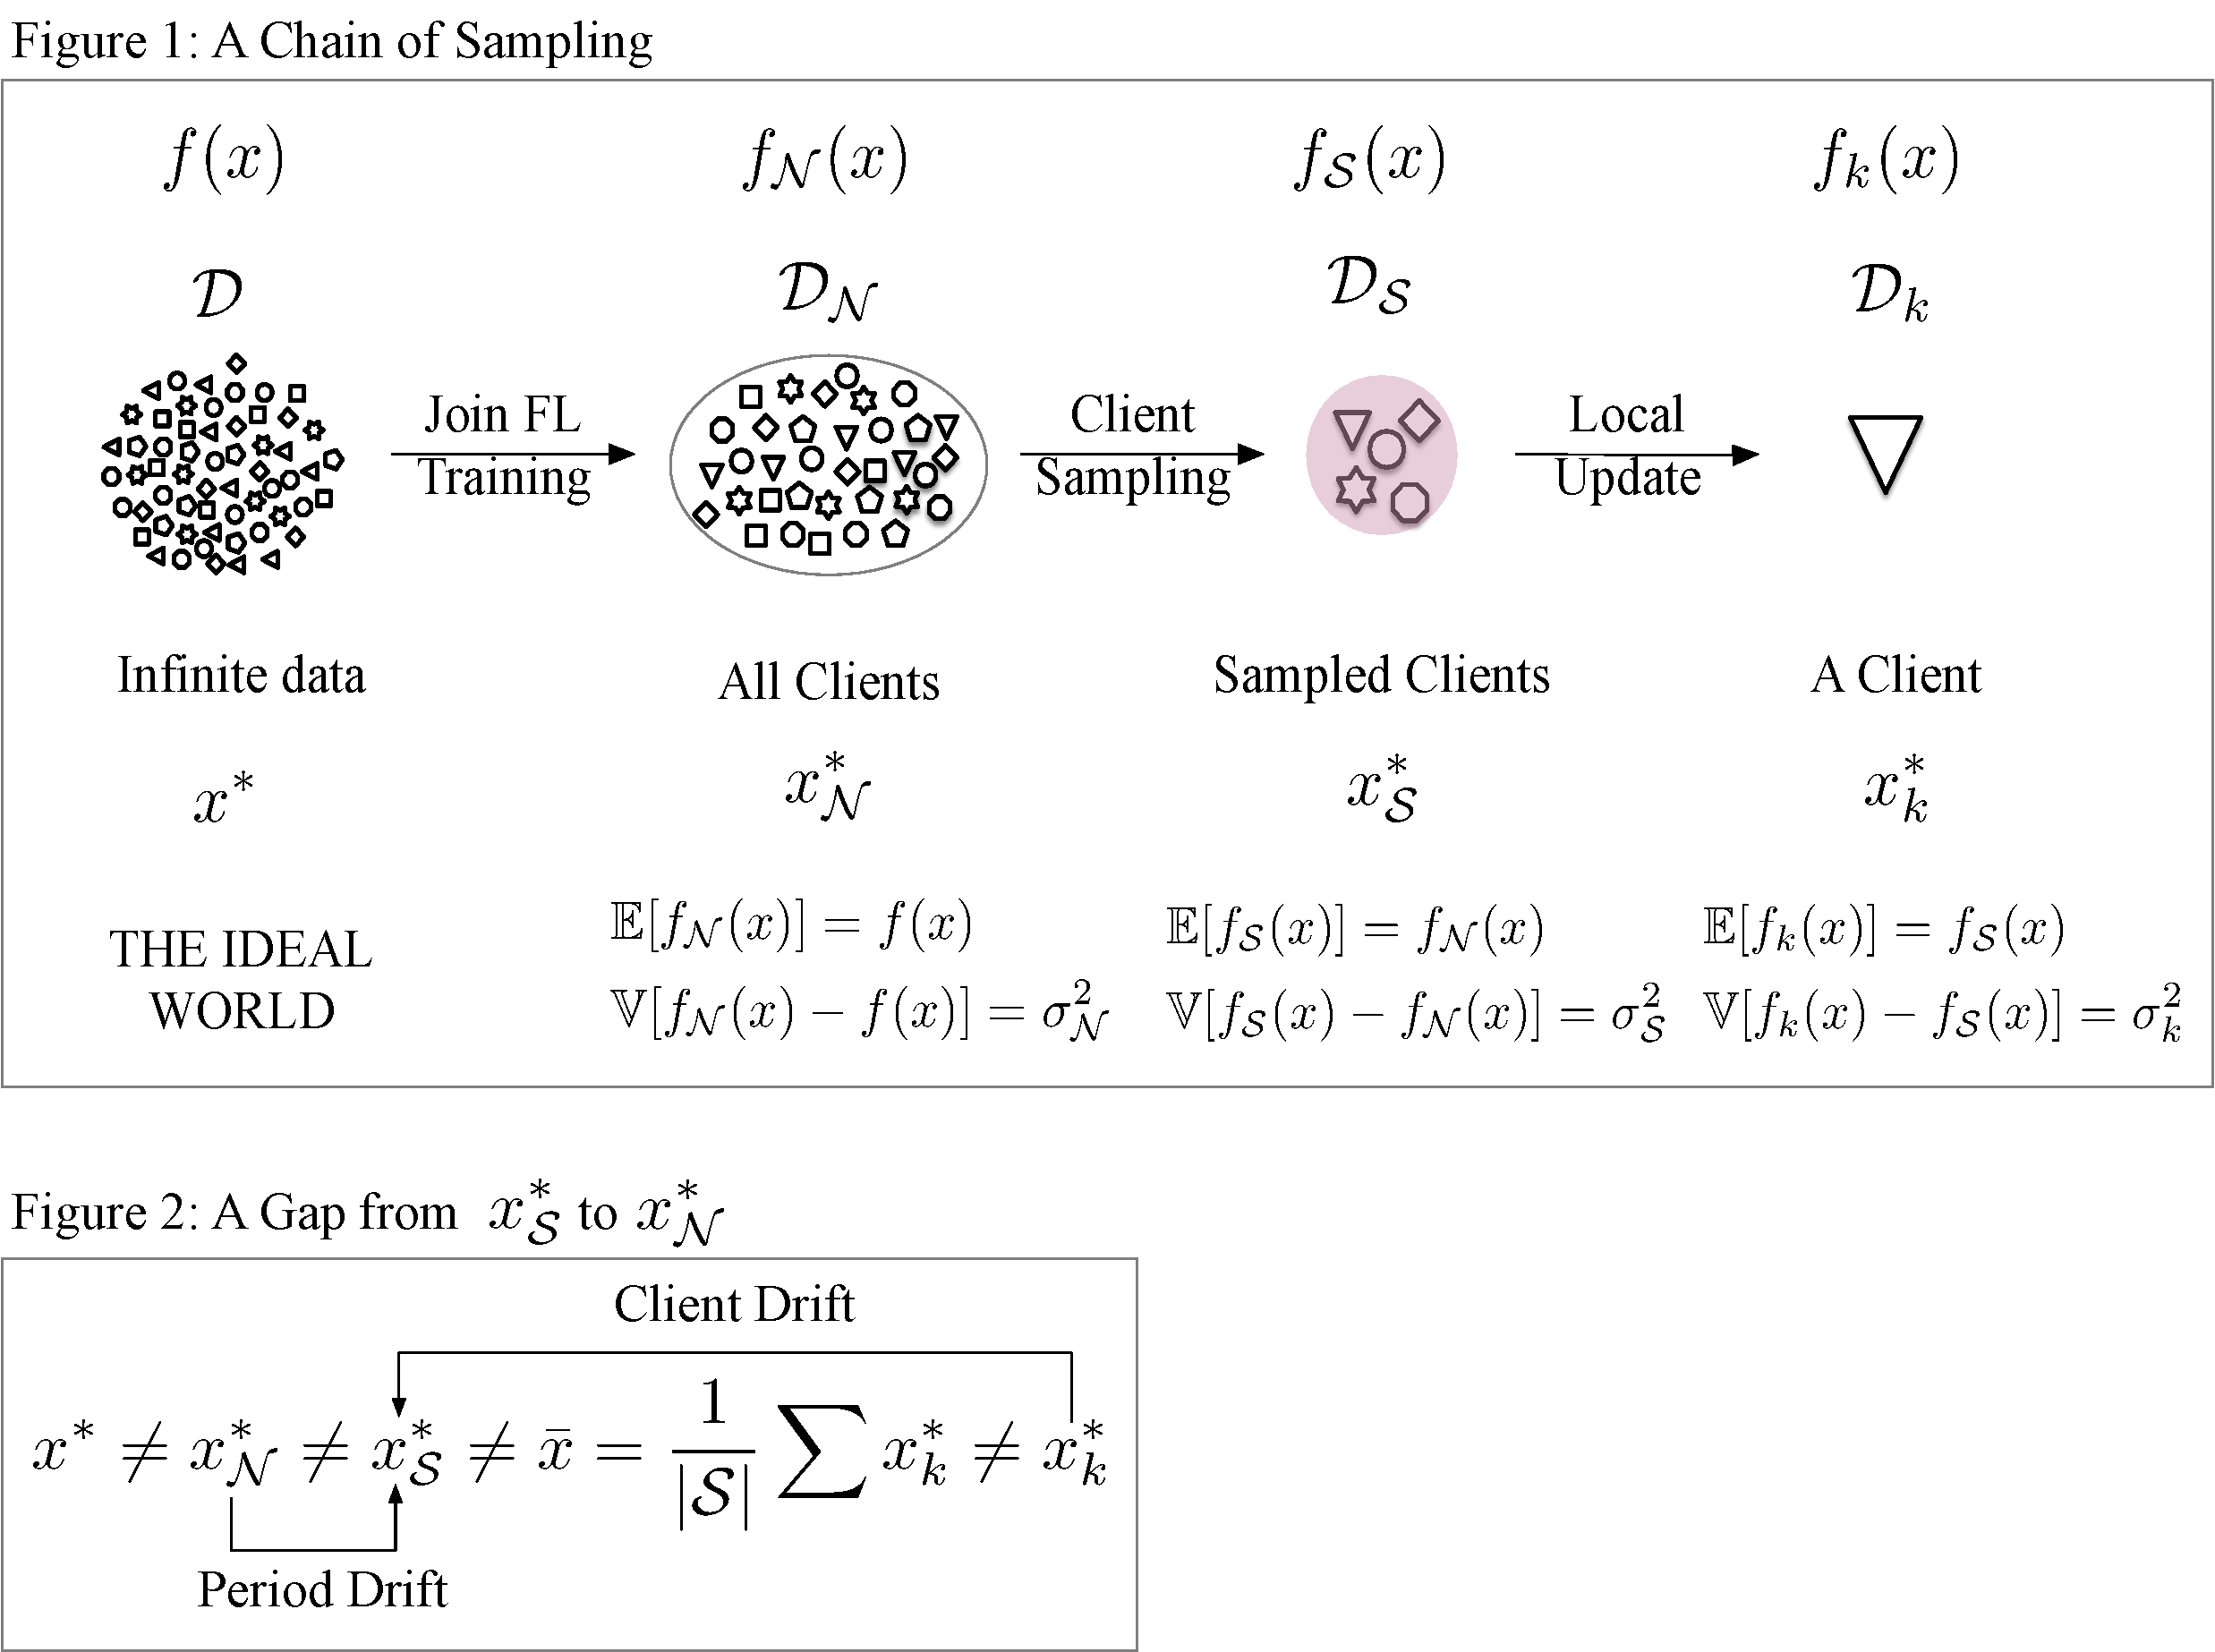
\includegraphics[width=0.8\linewidth]{drifts.pdf}
    \caption{\textbf{Illustration of period drift and client drift in the FL process.}}
    \label{fig:drifts}
\end{figure}

% the inequality $\frac{1}{S}\sum _ {i \in S}x _ i^* \neq x^*$ can be equated to (or entirely attributed to) the client drift, and whether it already includes the concept of "period drift". 

% To clarify the concept of "period drift" and "client drift" in FL, we refine the inequality $\frac{1}{S}\sum _ {i \in S}x _ i^* \neq x^*$ as $\frac{1}{S}\sum _ {i \in S}x _ i^* \neq x^*$ to $x^* \neq x _ {\mathcal{N}}^* \neq x _ {\mathcal{S}}^* \neq \bar{x} =\frac{1}{|\mathcal{S}|}\sum x _ k^*  \neq x _ k^*$. In FL, we are expecting to estimate the global optima $x^* _ {\mathcal{N}}$ (or the ideal optima $x^*$) through (weighted) averaging $\bar{x} =\frac{1}{|\mathcal{S}|}\sum x _ k^*$. However, in fact, this average $\bar{x}$ can only estimate $x^* _ {\mathcal{S}}$ and cannot estimate the global optima $x^* _ {\mathcal{N}}$ (see the lower part of Fig~\ref{fig:drifts}), due to the distribution difference between $\mathcal{D} _ \mathcal{S}$ (sampled from $\mathcal{D} _ \mathcal{N}$ and $\mathcal{D} _ \mathcal{N}$ itself can be arbitrarily large, and clients know nothing about the global distribution. 
% Essentially, we can only make estimates from our current sample set. Without specific information on the sampling of the previous level, we cannot determine the prior conditions or the original distribution of these samples. 
% Therefore, it is inappropriate to crudely attribute the inequality $\frac{1}{S}\sum _ {i \in S}x _ i^* \neq x^*$ entirely to client drift, as it also includes impacts unrelated to local updates, such as the generalization error $\sigma _ {\mathcal{N}}^2$ and client sampling $\sigma _ {\mathcal{S}}^2$. 
% Thus, it is more appropriate to represent client drift more precisely with $\bar{x} =\frac{1}{|\mathcal{S}|}\sum x _ k^* \neq x_{\mathcal{S}}^*$. An interesting counterexample is that if each client only performs one step of gradient update, there is no client drift, as the average of one step of gradient updates from different clients is just the gradient under the current batch, but the following inequality still holds $x^* \neq x _ {\mathcal{N}}^* \neq x _ {\mathcal{S}}^* = \bar{x} =\frac{1}{|\mathcal{S}|}\sum x _ k^*$, and the impact of period drift still exists. Therefore, the concept of period drift is completely independent of client drift.

To clarify the concepts of "period drift" and "client drift" in FL, we refine the commonly cited inequality \(\frac{1}{S}\sum_{i \in S}x_i^* \neq x^*\). We propose a more nuanced formulation: \(x^* \neq x_{\mathcal{N}}^* \neq x_{\mathcal{S}}^* \neq \bar{x} = \frac{1}{|\mathcal{S}|}\sum x_k^* \neq x_k^*\). 
In FL, the goal is to estimate the global optimum \(x^*_{\mathcal{N}}\)—or ideally, \(x^*\)—through the weighted average \(\bar{x} = \frac{1}{|\mathcal{S}|}\sum x_k^*\). However, this average \(\bar{x}\) often only approximates \(x^*_{\mathcal{S}}\) and falls short of estimating the true global optimum \(x^*_{\mathcal{N}}\) due to significant distributional discrepancies between \(\mathcal{D}_{\mathcal{S}}\) and \(\mathcal{D}_{\mathcal{N}}\). This variance is highlighted in the lower part of Figure \ref{fig:drifts} and illustrates the challenges in drawing reliable inferences about the global data distribution from locally sampled subsets.


Given that we only have data from current samples and lack comprehensive information about the broader sampling framework, it's clear that attributing the inequality \(\frac{1}{S}\sum_{i \in S}x_i^* \neq x^*\) solely to client drift is misleading. This inequality encompasses effects beyond local updates, including generalization error \(\sigma_{\mathcal{N}}^2\) and client sampling \(\sigma_{\mathcal{S}}^2\). 
A precise representation of client drift would therefore be \(\bar{x} = \frac{1}{|\mathcal{S}|}\sum x_k^* \neq x_{\mathcal{S}}^*\). An illustrative example of this is when each client performs a single gradient update step; there is effectively no client drift, as the average of these updates reflects the gradient of the current batch. Yet, the disparity \(x^* \neq x_{\mathcal{N}}^* \neq x_{\mathcal{S}}^* = \bar{x} = \frac{1}{|\mathcal{S}|}\sum x_k^*\) still persists, and the influence of period drift remains. Hence, period drift is fundamentally distinct from client drift and operates independently.



\section{The difference between \textit{Drift} in FL and the \textit{Noise} of centralized SGD}\label{appdx:analogy}

Federated learning possesses unique characteristics compared to traditional centralized optimization, such as client sampling, multiple local epochs, and non-iid data distribution. In this context, drifts in federated learning can be viewed as noises to the training dynamics. More specifically, period drift, originating from non-iid data and partial participation (only a subset of clients participate in each round), can be likened to the implementation of a mini-batch technique in the full-batch gradient descent of centralized training \citep{ziyin2021strength}. Here, the distinction is that in centralized optimization issues, each batch is iid, and each batch's data distribution closely mirrors the overall distribution, albeit with a noise component. This noise becomes remarkably pronounced in federated learning, given that client data is non-iid. Client drift, arising from non-iid data and multiple local updates (where each client runs local SGD with multiple steps), is a well-structured noise \citep{lin2018don}. Due to the combined impact of client drift and period drift, the situation can be perceived as adding a noise term to the original model (or gradient). The research outlined in this paper based on the difference between the drifts in federated learning and the noises in centralized SGD. 

\subsection{Visualization of difference between Period Drift and noise in SGD}
\label{sec:diff_rounds}

In this section, we provide a visualization to illustrate the fundamental difference between period drift in cross-device federated learning and the noise introduced by stochastic gradient descent (SGD). While both phenomena introduce stochasticity into the optimization process, their nature and impact on model convergence differ significantly.

Figure \ref{fig:diff_rounds} depicts this distinction by comparing the gradient directions across different communication rounds in federated learning. Period drift arises from the systematic shifts in client data distributions between communication rounds, creating consistent biases in gradient direction for extended periods. In contrast, SGD noise exhibits more random fluctuations that tend to average out over time.

\begin{figure}[h]
    \centering
    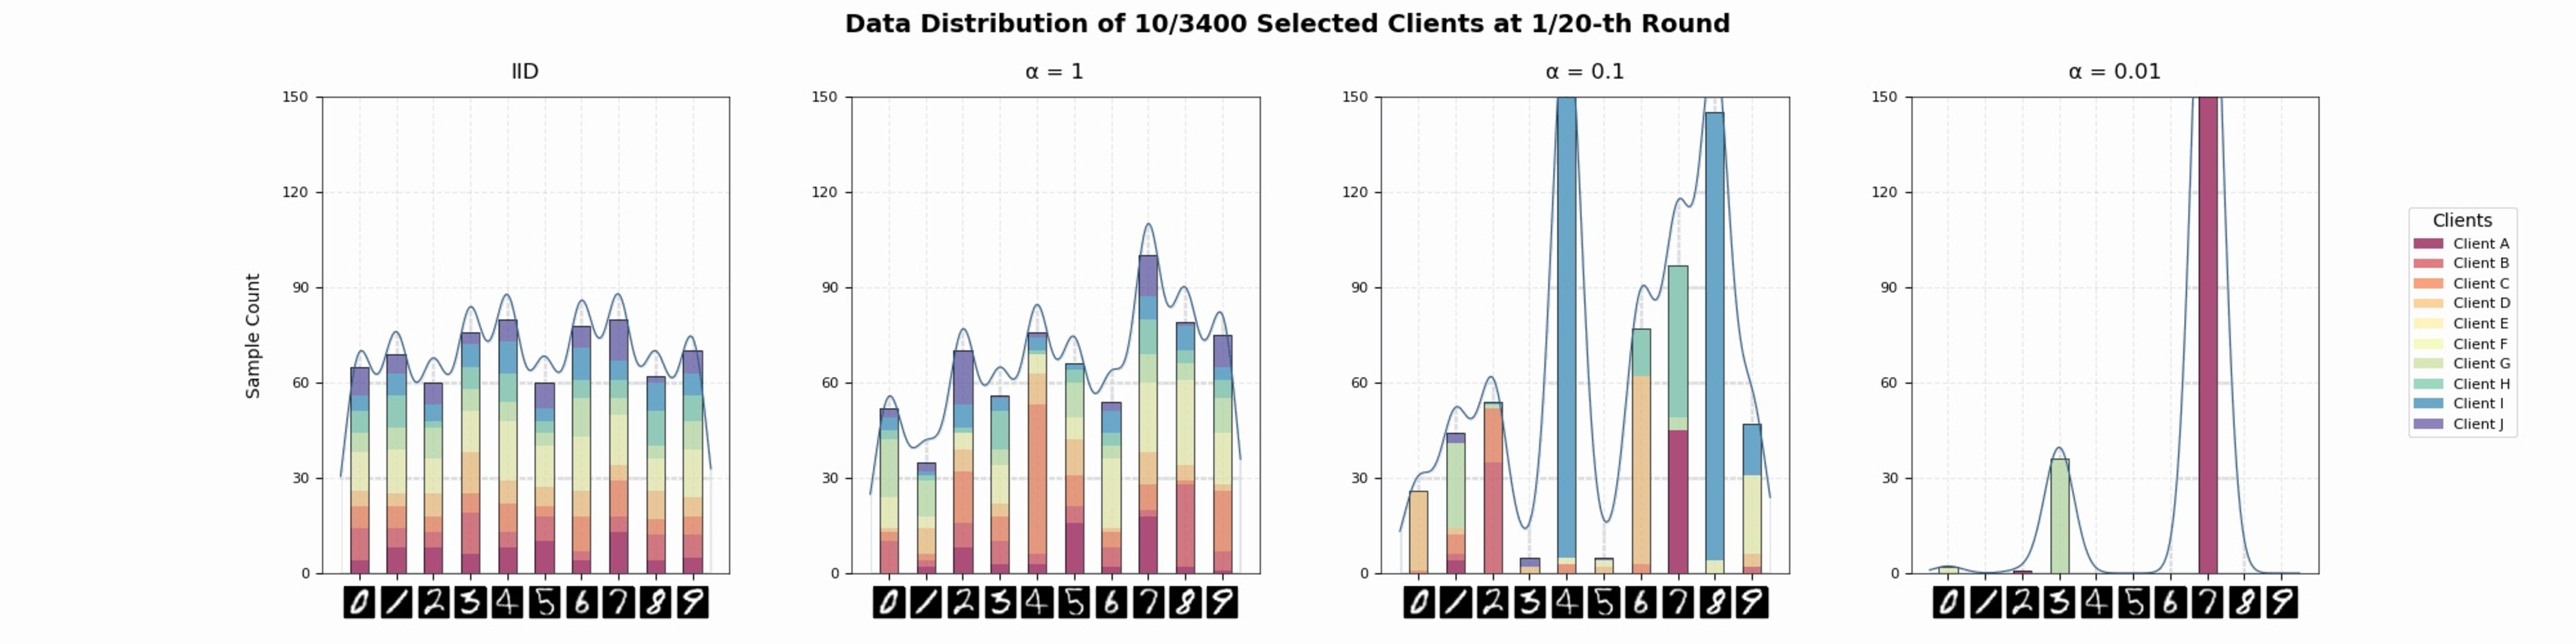
\includegraphics[width=0.8\linewidth]{diff_rounds.pdf}
    \caption{\small \textbf{Visualization of the difference between period drift and SGD noise}}
    \label{fig:diff_rounds}
\end{figure}

This visualization highlights why period drift poses a more significant challenge to federated learning than standard SGD noise. While SGD noise is often assumed to have zero mean and can be mitigated through increased batch sizes or adaptive optimization methods, period drift introduces differet kind of noise that depends on data heterogeneity that require specialized techniques like our proposed \fedeve algorithm to effectively address. The systematic nature of period drift makes it particularly problematic in highly heterogeneous cross-device settings, as demonstrated in our experimental results in Section \ref{sec:exp_setup}.

\subsection{A simple analysis of data heterogeneity and period drift}
Let us analyze how data heterogeneity impacts the data distribution difference between sampled clients and the overall population. We begin by examining the expectation of the sampled distribution $P_S$. Since clients are randomly selected, the expectation equals the overall data distribution:

\begin{equation}
    \mathbb{E}[P_S] = \mathbb{E}\left[ \frac{1}{|S|} \sum_{i \in S} D_i \right] = \frac{1}{|S|} \sum_{i=1}^{N} D_i = P
\end{equation}

Next, we calculate the variance of $P_S$. Using the linearity of variance and independence:

\begin{equation}
    \begin{aligned}
        \text{Var}(P_S) &= \text{Var}\left( \frac{1}{|S|} \sum_{i \in S} D_i \right) \\
        &= \frac{1}{|S|^2} \sum_{i \in S} \text{Var}(D_i) \\
        &= \frac{1}{|S|^2} \sum_{i \in S} \frac{1}{M} \sum_{j=1}^{M} (p_{ij} - p_j)^2
    \end{aligned}
\end{equation}

Since each client in $S$ is independently and identically distributed, taking the expectation yields:

\begin{equation}
    \mathbb{E}[\text{Var}(P_S)] = \frac{1}{|S|} \cdot \frac{1}{N} \sum_{i=1}^N \text{Var}(D_i) = \frac{H}{|S|}
\end{equation}

Finally, we derive the expectation of the data distribution difference between selected clients:

\begin{equation}
    \begin{aligned}
        \mathbb{E}[D_S] &= \mathbb{E}[\text{Var}(P_S, P)] \\
        &= \mathbb{E}\left[ \frac{1}{M} \sum_{j=1}^{M} \left( \frac{1}{|S|} \sum_{i \in S} p_{ij} - p_j \right)^2 \right] \\
        &= \frac{1}{M} \sum_{j=1}^{M} \mathbb{E}\left[ \left( \frac{1}{|S|} \sum_{i \in S} p_{ij} - p_j \right)^2 \right] \\
        &= \text{Var}(P_S) \\
        &= \frac{H}{|S|}
    \end{aligned}
\end{equation}

This result demonstrates that the expected data distribution difference among selected clients is directly proportional to the system's data heterogeneity $H$ and inversely proportional to the number of selected clients $|S|$. This finding has two important implications:

\begin{enumerate}
    \item As data heterogeneity $H$ increases, the expected data distribution difference among selected clients also increases. In the IID case where $H = 0$, we have $\mathbb{E}[D_S] = 0$, indicating that any client selection will match the overall distribution.
    \item As the number of selected clients $|S|$ increases, the expected data distribution difference decreases, suggesting that increasing participation can help mitigate the impact of data heterogeneity.
\end{enumerate}


\section{The relationship between period drift and client drift}

The relationship between period drift and client drift can be understood through their distinct yet interrelated effects on the FL optimization process. First, there is a clear sequential nature to these drifts - period drift occurs first in the optimization process, as it is determined by client selection at the beginning of each round. Client drift then follows as a consequence of local updates performed by the selected clients. This sequential relationship means that period drift can influence the magnitude and direction of subsequent client drift.

When data heterogeneity is high, period drift leads to biased optimization objectives for each round. This bias can be amplified by client drift during local updates, as clients further optimize towards their local objectives. The combination of these drifts results in increased variance in model updates, slower convergence rates, and potential divergence from the global optimum.
Despite their potentially harmful effects, these drifts can sometimes compensate for each other. Period drift may help prevent over-fitting to the data distribution of currently selected clients, while client drift can help explore the local optimization landscape more thoroughly. Additionally, the interaction between these drifts can create a natural regularization effect.
The magnitude of these drifts operates at different scales, which can be expressed mathematically as:
\begin{equation}
    \begin{aligned}
        \text{Period Drift} &\propto \frac{H}{|S|} \\
        \text{Client Drift} &\propto K \cdot H
    \end{aligned}
\end{equation}
where $H$ is the heterogeneity measure, $|S|$ is the number of selected clients, and $K$ is the number of local steps.
Understanding this relationship is crucial for designing effective FL algorithms that can handle both types of drift simultaneously, as addressing one type of drift in isolation may inadvertently exacerbate the other.



\subsection{The justification of Gaussian-like noise assumption \ref{assum:drift}}\label{sec:assum1_just}
% \newtheorem*{assumption*}[theorem]{Assumption}
\begin{assumption}[\ref{assum:drift}]
   \textit{The aggregated model parameters on the server $w_{server}$, can be represented as the sum of the optimal parameters $w^*$ and a drift (noise) that follows a normal distribution ${w}_{drift} \sim \mathcal{N}(0,\sigma_{drift}^2)$:}
   \begin{equation}
      {w}_{server}={w}^*+{w}_{drift}\leftarrow noise,
   \end{equation}
\end{assumption}
% \begin{equation}\label{eq:drift}
%    {w}_{server}={w}^*+{w}_{drift}\leftarrow noise,
% \end{equation}
where $w^*$ represents the optimal parameters obtained through the use of stochastic gradient descent (SGD), $w_{drift}$ represents the noise term caused by factors such as client sampling, multiple local epochs, and non-iid data distribution that we assume a normal distribution, and $w_{server}$ represents the aggregated model parameters also follows a normal distribution ${w}_{server} \sim \mathcal{N}(w^*,\sigma_{drift}^2)$, with the expectation of the aggregate model parameters being equal to the optimal parameters, i.e. $\mathbb{E}[{w}_{server}]={w}^*$. 

% In this paper, we represent the aggregated model parameters on the server as the sum of the optimal parameters and a drift (noise): $w_{server}=w^*+w_{drift}$, and assume that $w_{drift}$ follows a normal distribution. We justify this assumption by demonstrating its prevalence, and explaining it in FL.

% On the one hand, modeling noise in dynamic systems as a Gaussian (normal) distribution is a widespread practice with a long history, dating back to the 1940s \citep{kramers1940brownian}. The majority of prior works analyzing the behavior of SGD optimization argue that the noise on gradients or parameters is Gaussian [2-8]. Wu et al. [6] rationalize the assumption of Gaussianity for SGD noise, stating that limit theorem theory ensures the convergence of SGD noise to a specific infinite divisible distribution, which belongs to the Gaussian class if the noise's second moment is finite (Lindeberg's condition). Although it has been argued that maybe the noise in SGD is better characterized by $S\alpha S$ noise [9], this argument was refuted and redirected to the previously proposed Gaussian noise model [7, 10].

% On the other hand, we explain the principle of Gaussian noise in FL. The Lindeberg-Feller Central Limit Theorem (CLT) [11] is a fundamental reason for the prevalence of normal distribution. The CLT states that the sum (or average) of random variables converges toward a normal distribution, regardless of the distributions of these random variables themselves. In FL, noise may arise due to client sampling (period drift), and multiple local updates (client drift). The observed drifted model $w_{server}$ typically results from the superimposition of these factors, making normal distribution an appropriate model for describing the noise. In fact, the model averaging of FedAvg inherently satisfies the CLT conditions, as $w_{server}= \bar{w}= \frac{1}{n}\sum_{i=1}^n w_i$. This implies that, regardless of the distributions of $w_i$, $\bar{w}$ always follows a normal distribution (explains the Gaussian client drift $f$). Besides, as stated in [6], if the sampling noise belongs to the Gaussian class, then the gradient noise is also Gaussian (explains the Gaussian period drift $Q$).

In this paper, we conceptualize the aggregated model parameters on the server as the summation of optimal parameters and a certain drift (or noise), represented as: $w_{server}=w^*+w_{drift}$. We also assume that $w_{drift}$ is subject to a normal (Gaussian-like) distribution, and justify this assumption by demonstrating its prevalence, and explaining it in FL.

From a historical standpoint, modeling noise in dynamic systems as a Gaussian-like distribution is a widely accepted practice. This dates back to \citep{kramers1940brownian}, and many studies analyzing Stochastic Gradient Descent (SGD) optimization have emphasized the Gaussian nature of noise on gradients or parameters \citep{mandt2017stochastic,zhu2019anisotropic,simsekli2019tail,ziyin2021strength}.  This assumption of Gaussianity for SGD noise is justified by \citet{wu2020noisy}, which guarantees the SGD noise's convergence to a specific infinite divisible distribution. This falls under the Gaussian class provided the noise's second moment is finite (as per Lindeberg's condition). While it has been proposed that the noise in SGD might be better represented by $S\alpha S$ noise \citep{simsekli2019tail}, this idea has been challenged and redirected back to the earlier proposed Gaussian noise model \citep{zhekexie2021a, battash2023revisiting}.

We further elucidate the occurrence of Gaussian noise in the context of FL. The Lindeberg-Feller Central Limit Theorem (CLT) \citep{lindeberg1922neue} plays a key role in explaining the prevalence of the normal distribution. It posits that the sum (or average) of random variables gravitates towards a normal distribution (no need to assume iid of these random variables themselves), irrespective of the individual distributions of these variables. In FL, the emergence of noise can be attributed to partial participation (referred to as period drift) and multiple local updates (referred to as client drift). The drifted model that we observe, $w_{server}$, is typically the result of the combination of these factors, making the normal distribution an apt model for characterizing the noise. 
% Importantly, the model averaging process inherent to FedAvg aligns with the conditions of the CLT, as demonstrated by the equation $w_{server}= \bar{w}= \frac{1}{n}\sum_{i=1}^n w_i$. This implies that despite the varying distributions of $w_i$, the $\bar{w}$ will always follow a normal distribution, thereby explaining the Gaussian nature of client drift ($f$). 
% Moreover, as per the assertion in \citet{wu2020noisy}, if the sampling noise is of the Gaussian class, the gradient noise will also follow the Gaussian distribution, thereby accounting for the Gaussian period drift ($Q$).


\textbf{The impact of noise on generalization}
In order to investigate the effect of the deviation on performance in FL, we utilize a regression optimization objective as in previous studies, such as \citep{zhang2019lookahead} and \citep{wu2018understanding}:
$$
\hat{\mathcal{L}}({w})=\frac{1}{2}({w}+{w}_{drift})^T {A}({w}+{w}_{drift}),
$$
where ${w}_{drift} \sim \mathcal{N}(0,\sigma^2)$ is the drift caused by the characteristics of FL. Therefore, the generalization error can be formulated as:
\begin{equation*}
   \begin{aligned}
      \mathcal{L}\left(w^{t}\right)&=\mathbb{E}\left[\hat{\mathcal{L}}\left(w^{t}\right)\right]=\frac{1}{2} \mathbb{E}\left[\sum_i a_i\left(w_i^{t^2}+\textcolor{red}{\sigma_i^2}\right)\right]\\
      &=\frac{1}{2} \sum_i a_i\left(\mathbb{E}\left[w_i^{t}\right]^2+\mathbb{V}\left[w_i^{t}\right]+\textcolor{red}{\sigma_i^2}\right),
   \end{aligned}
\end{equation*}
where $A$ is the matrix of quadratic form of the MSE loss function, and $a_i$ is the elements of $A$. As results, the generalization error can also be decomposed into three components: bias, variance, and noise. The noise component in FL context is further influenced by factors such as client sampling, multiple local epochs, and non-iid data distribution, leading to a much larger overall generalization error compared to centralized SGD. This formulation reveals the reason of why FL usually performs worse than centralized training. Thus, our goal is to reduce the variance of drift $\sigma^2$ in order to improve both the convergence and performance of the model.

\subsection{The justification of independence assumption \ref{assum:wqr} of client drift and period drift}\label{sec:assum2_just}
\begin{assumption}[\ref{assum:wqr}]
   \textit{The initialization model parameters are independent of all period drifts $Q_t$ and client drifts $R_t$ at each communication round, that is $w_0 \perp Q_0, Q_1,\cdots, Q_t$ and $w_0 \perp R_0,  R_1,\cdots, R_t$.}
\end{assumption}

This assumption can be justified from various perspectives, demonstrating its reasonableness:
\begin{itemize}[leftmargin=*,nosep]
   \item \textbf{Independence of the initial model parameters from other noise variables:} This assumption suggests that there is no direct relationship between the initial model parameters ($w_0$) and period drifts or client drifts. This is a reasonable assumption since initial model parameters are typically determined prior to training and hence are not influenced by any noise processes.
   \item \textbf{Independence of client drifts between each communication round:} According to this assumption, client drifts ($R_0, R_1, \cdots, R_t$) in different communication rounds are independent of each other. The client drift is influenced by data heterogeneity and multiple local updates. A higher degree of data heterogeneity and an increased number of local updates can result in greater client drift. Each client has its own fixed client drift\citep{guo2021towards}, and the client drift in each communication round doesn't impact other rounds, the assumption of client drift independence is reasonable. 
   \item \textbf{Independence of period drifts between each communication round:} This assumption contends that the period drifts ($Q_0, Q_1, \cdots, Q_t$) across different communication rounds are independent. Period drift is influenced by data heterogeneity and client sampling. Though period drift may be caused by biased client sampling due to factors like time and geographic locations, leading to a dependence between period drifts in different communication rounds, this paper considers the case where random client sampling occurs in each communication round. Here, one round of client sampling doesn't affect others, thus rendering the independence of period drift reasonable.
   \item \textbf{Independence between period drifts and client drifts at each communication round:} This assumption argues that the client drifts ($R_0, R_1, \cdots, R_t$) and the period drifts ($Q_0, Q_1, \cdots, Q_t$) at each communication round are independent. While both client drift and period drift are influenced by data heterogeneity, they are conditionally independent given the heterogeneous data. We offer a causal graph to depict their relationships:
    \begin{center}
      multiply local updates $\longrightarrow$  client drift $\longleftarrow$ data heterogeneity $\longrightarrow$ period drift $\longleftarrow$  client sampling
   \end{center}
   This graph indicates that data heterogeneity is a common cause of client drift and period drift, and varying levels of data heterogeneity result in different magnitudes of client drift and period drift. However, given that the heterogeneous data is constant across clients (i.e., given D), we can express P(client drift, period drift|D) = P(client drift|D) * P(period drift|D). Indeed, conditioning on a given heterogeneous data set is a fundamental assumption in Federated Learning.
\end{itemize}

\paragraph{Empirical Analysis}
% Thank you for your instructive suggestion to justify the Gaussian noise assumption empirically. 
To verify that both period drift and client drift adhere to the Gaussian assumption, we design this experiment by means of randomly selecting a model parameter and tracing its period drift and client drift across the subsequent 1500 rounds of training. 
During this process, we collected the global optima $x _ {\mathcal{N}}^*$ of global objective on the whole training dataset for each communication round, as well as the optima $x _ {\mathcal{S}}^*$ on the dataset of sampled clients for each communication round, and the local optima $x _ k^*$ of the dataset of a single client, respectively. 
The period drift is represented by $x _ {\mathcal{S}}^*-x _ {\mathcal{N}}^*$, while the client drift is depicted by $x _ {k}^*-x _ {\mathcal{S}}^*$. The sampling results are visualized using histograms. 
Experiments were conducted with alpha values in the scope $\alpha=[1,0.1,0.01]$, as illustrated in Fig~\ref{fig:gaussian}. We also employ the `normaltest` function from `scipy.stats`, utilizing the *D'Agostino-Pearson Test* to determine if a sample deviates from a normal distribution. Here, a p-value $>$ 0.05 indicates conformity to a normal distribution. 
The experimental results showed that both period drift and client drift follow a normal distribution, confirming the reliability of the Gaussian distribution assumption.
% Your instructive suggestion really helps us improve the paper, and we sincerely appreciate that you could consider improving your score if there is no further concern.


\begin{figure}[h]
    \centering
    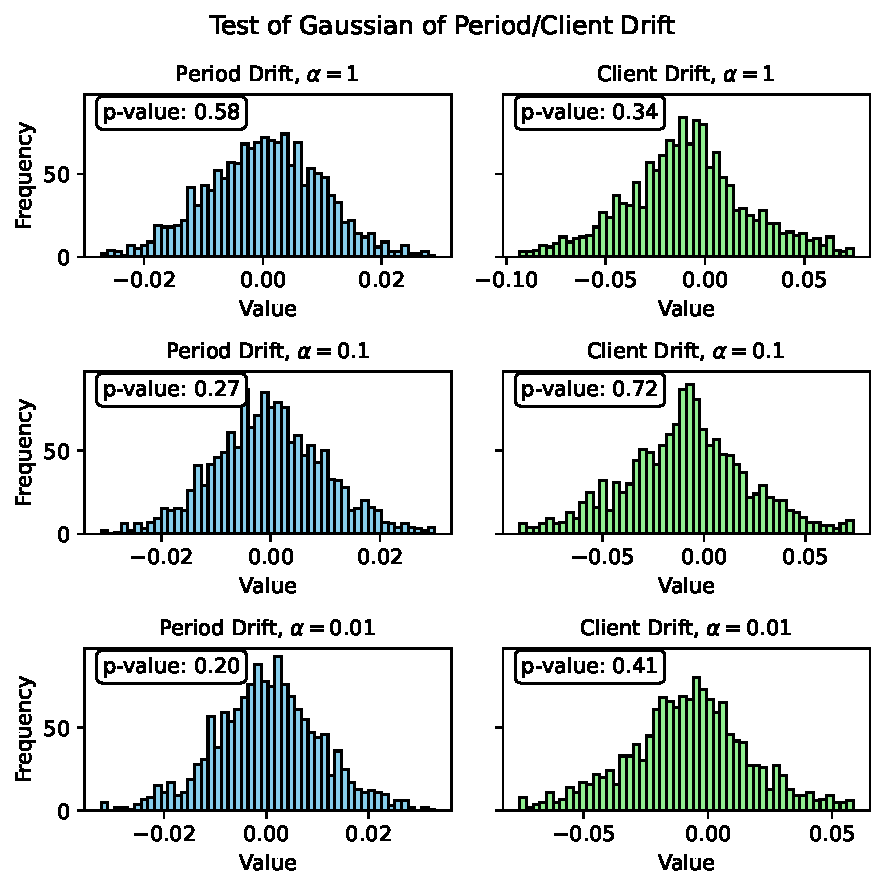
\includegraphics[width=0.8\linewidth]{gaussian.pdf}
    \caption{\textbf{Empirical justification of Gaussian distribution assumption.}}
    \label{fig:gaussian}
\end{figure}



\subsection{The Independence of Noise}\label{appdx:noise}
\begin{lemma}[\ref{lemma:independence_noise}]
   \textit{(Independence of Noise). the noise present in the prediction and observation at each communication round is independent of the current state of the model, specifically, $w_t \perp Q_t$ and $w_t \perp R_t$.}
\end{lemma}

% \textit{Proof:} The proof of independence can be established by examining the relationship between $w_{t+1}$ and $Q_t$ and $R_t$. In the given scenario, $w_t$ denotes the state of the model at round $t$. $Q_t$ and $R_t$ are the noise in the prediction and observation respectively, at each communication round $t$. Since $w_{t+1}$ is related to the $Q_t$ and $R_t$, by expressing the state transfer function as $w_{t+1}=T_t(w_t,Q_t,R_t)$ at the $t$-th round, it can be further shown that
% \begin{equation}
%    \begin{aligned}
%       w_{t}&=T_{t-1}(w_t,Q_{t-1},R_{t-1}),\\
%       w_{t-1}&=T_{t-2}(w_t,Q_{t-2},R_{t-2}),\\
%       &\vdots \\
%       w_{2}&=T_{1}(w_1,Q_{1},R_{1}),\\
%       w_{1}&=T_{0}(w_0,Q_{0},R_{0}),\\
%    \end{aligned}
% \end{equation}
% and so on, leading to the equation $w_{t}=T(w_0,Q_0,Q_1,\cdots,Q_{t-1},R_0,R_1,\cdots,R_{t-1})$. The proof proceeds by establishing a chain of dependencies between $w_{t+1}$ and $Q_t$ and $R_t$. You express $w_{t+1}$ as a function $T_t(w_t,Q_t,R_t)$, where $T_t$ is the state transition function at round $t$.
% Under the assumption of independence in the noise, it can be inferred in Assumption \ref{assum:wqr} that $w_0 \perp Q_0 \perp Q_1 \perp \cdots Q_t \perp R_0 \perp R_1 \perp \cdots R_t$. these parameters are all independent of each other at each round and are also independent of the initial parameters of the model. This means that they do not affect each other; the value of one does not influence or depend on the value of the others. Therefore, $W_t$ is independent of $Q_t$ and $R_t$, i.e. $W_t\perp Q_t\perp R_t$.

To prove this, we will first need to understand the relationship between the variables $w_{t+1}$, $Q_t$, and $R_t$.
In the given context, $w_{t+1}$ represents the state of the model at a particular communication round (say, round $t+1$). It is affected by the values of the period drift ($Q_t$) and client drift ($R_t$) at the previous round. This is represented by the state transfer function $w_{t+1}=T_t(w_t,Q_t,R_t)$.
However, this relationship does not imply that $w_{t+1}$ is dependent on $Q_t$ or $R_t$. To see why, let's look at how $w_t$ is formed. Using the state transfer function, we can express $w_t$ as:
\begin{equation}
\begin{aligned}
w_{t}&=T_{t-1}(w_{t-1},Q_{t-1},R_{t-1}),\\
w_{t-1}&=T_{t-2}(w_{t-2},Q_{t-2},R_{t-2}),\\
&\vdots \\
w_{2}&=T_{1}(w_{1},Q_{1},R_{1}),\\
w_{1}&=T_{0}(w_0,Q_{0},R_{0}),\\
\end{aligned}
\end{equation}
From this chain of equations, it is evident that $w_t$ is not only a function of the current round's period drift $Q_t$ and client drift $R_t$, but also of their past values and the past values of $w_t$ itself. In a more generalized form, we can write this as: $w_{t}=T(w_0,Q_0,Q_1,\cdots,Q_{t-1},R_0,R_1,\cdots,R_{t-1})$. Assumption \ref{assum:wqr} states that the period drift and client drift are independent of each other at each communication round and also independent of the initial model parameters. That is, $w_0 \perp Q_0 \perp Q_1 \perp \cdots Q_t \perp R_0 \perp R_1 \perp \cdots R_t$.
This assumption implies that the previous states of $w_t$ ($w_{t-1}$, $w_{t-2}$, and so on) do not have any influence on the current values of $Q_t$ and $R_t$. In other words, the noise present at each round is independent of the model's current state. Thus, $w_t$ is independent of $Q_t$ and $R_t$, denoted as $w_t\perp Q_t\perp R_t$.
Therefore, it can be concluded that the noise present in the prediction and observation at each communication round is indeed independent of the current state of the model, thereby confirming the independence of noise.
This statement about the independence of noise is significant because it confirms that the noise encountered during each communication round does not affect the model's state. This means that the model is robust and not affected by random perturbations, which is a desirable property in any machine learning model.

\subsection{Analysis of Kalman Gain in \fedeve} 
We conducted an in-depth analysis of the Kalman Gain $K$ 
\begin{figure}
  \centering
  \label{fig:kalman_gain}
  \includegraphics[width=\linewidth]{fedeve_Kalman.pdf}
  \caption{\small\textbf{Boxplots for Kalman Factors}}
\end{figure}
% \begin{figure}[ht]
%   \centering
%   % %\vspace{-4mm}
%   \includegraphics[width=\linewidth]{fedeve_Kalman.pdf}\label{fig:kalman_gain}
%   %\vspace{-6mm}
%   \caption{\small\textbf{Boxplots for Kalman Factors}}
%   %\vspace{-5mm}
%   \end{figure}
 of FedEve under various experimental settings, incorporating four levels of data heterogeneity and various local epochs, as shown in Figure 4. We observed that as data heterogeneity increases (i.e., as the value of $\alpha$ decreases), the Kalman Gain $K$ progressively enlarges. With the rise of data heterogeneity, the period drift starts to play a more dominant role. In this context, the primary role of Kalman Gain $K$ is to adjust the weights between global and local updates, as depicted by Equation (\ref{step:pre_s}) and (\ref{step:G_kal}). Further, according to Equation (\ref{step:M}), the model update tends to trust local updates more, stabilizing the optimization process. For varied counts of local updates, the relative change in Kalman Gain $K$ is marginal. This is primarily because, in cross-device FL, the client drift is not a pivotal or dominant factor, which aligns with our prior analysis in Figure \ref{fig:visualize}.


\subsection{Model Update with Bayesian filter}\label{appdx:bayesian}
\subsubsection{Bayesian filter}
This section begins by describing the main idea behind the approach: the combination of prediction and observation models using a Bayesian filter, which is a statistical tool for estimating an unknown probability density function (PDF) based on observations. The prediction process is explained using the concept of cumulative distribution functions (CDFs), which are functions giving the probability that a random variable is less than or equal to a certain value. The prediction process is characterized by the distribution:
\begin{equation}
   \begin{aligned}
   F_{\hat{w}_{t+1}}^{-}(w) &=P\left(\hat{w}_{t+1} \leq w\right) \\
   &=\sum_{u=-\infty}^w P\left(\hat{w}_{t+1}=u\right)\\
   &=\sum_{u=-\infty}^w \sum_{v=-\infty}^{+\infty} P\left(\hat{w}_{t+1}=u \mid w_t=v\right) P\left(w_t=v\right)\\
   &=\sum_{u=-\infty}^w \sum_{v=-\infty}^{+\infty} P\left[\hat{w}_{t+1}-f\left(w_t\right)=u-f(v) \mid w_t=v\right] P\left(w_t=v\right)\\
   &=\sum_{u=-\infty}^w \sum_{v=-\infty}^{+\infty} P\left[Q_t=u-f(v) \mid w_t=v\right] P\left(w_t=v\right)  \quad \Rightarrow \text{Prediction Equation} \\
   &=\sum_{u=-\infty}^w \sum_{v=-\infty}^{+\infty} P\left[Q_t=u-f(v)\right] P\left(w_t=v\right) \quad \Rightarrow \text{Lemma (\ref{lemma:independence_noise}}) \\
   &=\sum_{u=-\infty}^w\left\{\lim _{\epsilon \rightarrow 0} \sum_{v=-\infty}^{+\infty} f_{Q_t}[u-f(v)] \cdot \epsilon \cdot f_{w_t}^{+}(v) \cdot \epsilon\right\}\\
   &=\sum_{u=-\infty}^w\left\{\lim _{\epsilon \rightarrow 0} \int_{-\infty}^{+\infty} f_{Q_t}[u-f(v)] f_{w_t}^{+}(v) \mathrm{d} v \cdot \epsilon\right\}\\
   &=\int_{-\infty}^w \int_{-\infty}^{+\infty} f_{Q_t}[u-f(v)] f_{w_t}^{+}(v) \mathrm{d} v \mathrm{~d} u\\
   &=\int_{-\infty}^w \int_{-\infty}^{+\infty} f_{Q_t}[w-f(v)] f_{w_t}^{+}(v) \mathrm{d} v \mathrm{~d} w
   \end{aligned}
   \end{equation}
The first three steps apply the definition of the cumulative distribution function (CDF), which is the sum of probabilities up to a certain point. In the fourth step, the change of variables is used to switch from $u$ to $v$. The fifth and sixth steps apply Lemma \ref{lemma:independence_noise}, which states that the drift is independent of the weights $w_t$. The last three steps show how to convert the sum to an integral, which is a common method in probability theory for dealing with continuous random variables. Finally, the PDF of the prediction is obtained by taking the derivative of the CDF, which can be expressed as:
\begin{equation}\small
   f_{\hat{w}_{t+1}}^{-}(w)=\frac{\mathrm{d} F_{\hat{w}_{t+1}}^{-}(w)}{\mathrm{d} w}=\int_{-\infty}^{+\infty} f_{Q_t}[w-f(v)] f_{w_t}^{+}(v) \mathrm{d} v
\end{equation}
The observation process is also characterized by a PDF. Similar steps are used to manipulate and simplify the expression for the PDF of the observed value $w_{t+1}$, given the predicted value $\hat{w}_{t+1}$. Specifically:
\begin{equation}
   \begin{aligned}
   &f_{\tilde{w}_{t+1} \mid \hat{w}_{t+1}}\left(w_{t+1} \mid w\right)=\lim _{\epsilon \rightarrow 0} \frac{F_{\tilde{w}_{t+1} \mid \hat{w}_{t+1}}\left(w_{t+1}+\epsilon \mid w\right)-F_{\tilde{w}_{t+1} \mid \hat{w}_{t+1}}\left(w_{t+1} \mid w\right)}{\epsilon}\\
   &=\lim _{\epsilon \rightarrow 0} \frac{P\left(w_{t+1} \leq \tilde{w}_{t+1} \leq w_{t+1}+\epsilon \mid \hat{w}_{t+1}=w\right)}{\epsilon} \\
   &=\lim _{\epsilon \rightarrow 0} \frac{P\left[w_{t+1}-h(w) \leq \tilde{w}_{t+1}-h\left(\hat{w}_{t+1}\right) \leq w_{t+1}-h(w)+\epsilon \mid \hat{w}_{t+1}=w\right]}{\epsilon}\\
   &=\lim _{\epsilon \rightarrow 0} \frac{P\left[w_{t+1}-h(w) \leq R_t \leq w_{t+1}-h(w)+\epsilon \mid \hat{w}_{t+1}=w\right]}{\epsilon} \Rightarrow \text{Lemma (\ref{lemma:independence_noise})}\\
   &=\lim _{\epsilon \rightarrow 0} \frac{F_{R_t}\left[w_{t+1}-h(w)+\epsilon\right]-F_{R_t}\left[w_{t+1}-h(w)\right]}{\epsilon}\\
   &=f_{R_t}\left[w_{t+1}-h(w)\right].
   \end{aligned}
   \end{equation}
The first two steps apply the definition of the probability density function (PDF), which is the derivative of the cumulative distribution function (CDF). The third and fourth steps use a change of variables to express the PDF in terms of the difference between the observed and predicted values. The fifth step applies the independence Lemma (\ref{lemma:independence_noise}) to simplify the conditional probability. The sixth step calculates the limit to arrive at the PDF of the observation process.
As a consequence of combining the prediction and observation distributions, a fused model can be obtained, which can be described by its own probability density function (PDF) as:
\begin{equation}
   f_{w_{t+1}}^{+}(w)=\eta_t \cdot f_{\tilde{w}_{t+1} \mid \hat{w}_{t+1}}\left(\tilde{w}_{t+1} \mid \hat{w}_{t+1}\right) \cdot f_{\hat{w}_{t+1}}^{-}(w)=\eta_t \cdot f_{R_t}\left[\tilde{w}_{t+1}-h(\hat{w}_{t+1})\right] \cdot f_{\hat{w}_{t+1}}^{-}(w),
\end{equation}
where 
\begin{equation}
    \small
   \eta_t=\left[\int_{-\infty}^{+\infty} f_{\tilde{w}_{t+1} \mid \hat{w}_{t+1}}\left(\tilde{w}_{t+1} \mid \hat{w}_{t+1}\right) f_{\hat{w}_{t+1}}^{-}(w) \mathrm{d} w\right]^{-1}=\left\{\int_{-\infty}^{+\infty} f_{R_t}\left[\tilde{w}_{t+1}-h(\hat{w}_{t+1})\right] f_{\hat{w}_{t+1}}^{-}(w) \mathrm{d} w\right\}^{-1}.
\end{equation}
The PDF of the fused model is obtained by multiplying the PDFs of the prediction and observation processes, normalized by a factor $\eta_t$.
The process of updating the fused model, also known as the Bayesian filter, can be summarized in the following steps:
\begin{equation}
   \begin{aligned}
   f_{w_t}^{+}(w) &\stackrel{\text {predict}}{\Longrightarrow} f_{\hat{w}_{t+1}}^{-}(w)=\int_{-\infty}^{+\infty} f_{Q_t}[w-f(v)] f_{w_t}^{+}(v) \mathrm{d} v\\ &\stackrel{\text {observe}}{\Longrightarrow} f_{w_{t+1}}^{+}(w)=\eta_t \cdot f_{R_t}\left[w_{t+1}-h(w)\right]
   \cdot f_{\hat{w}_{t+1}}^{-}(w),
   \end{aligned}
   \end{equation}
where $\eta_t=\left\{\int_{-\infty}^{+\infty} f_{R_t}\left[\tilde{w}_{t+1}-h(\hat{w}_{t+1})\right] f_{\hat{w}_{t+1}}^{-}(w) \mathrm{d} w\right\}^{-1}$. The fused model combines the prediction and observation distributions, and it describes the sequential steps of the Bayesian filter: starting with the PDF at time $t$, a prediction is made for the PDF at time $t+1$, and then this prediction is updated based on the observation to obtain the PDF at time $t+1$. The final estimation of the parameter can be obtained as a result of these update steps and can be represented as:
\begin{equation}
   \hat{w}_{t+1}=E\left[f_{w_{k+1}}^{+}(w)\right]=\int_{-\infty}^{+\infty} w f_{w_{k+1}}^{+}(w) \mathrm{d} w,
   \end{equation}
which is done by calculating the expected value of the PDF at time $t+1$. This is performed by multiplying the parameter $w$ by its probability density and integrating over all possible values of $w$. The integral provides a single, average value for $w$ weighted by its probability density, which serves as the final estimate of the parameter.

\subsubsection{\fedeve}\label{sec:fedeve}
% In this section, we demonstrate the derivation of the \fedeve algorithm from the Bayesian filter. The model update process in \fedeve is outlined as follows:

% \begin{align}
%    &\hat{w}_{t+1}=w_t-\eta_g M_t,\\
%    &\hat{\sigma}^2_{t+1}=\sigma^+_{t}+\sigma_{Q_t}^2,\\
%    & K=\frac{\hat{\sigma}^2_{t+1}}{\hat{\sigma}^2_{t+1}+\sigma_{R_t}^2},\\
%    & M_{t+1}= M_{t}+K(\Delta \tilde{w}_{t}-M_{t}),\\
%    & w_{t+1}=w_t-\eta_g M_{t+1},\\
%    &{\sigma}^2_{t}=(1-K)\hat{\sigma}^2_{t+1}.
% \end{align}

% It is important to note that the proof provided here is facilitated by the assumption of normal distribution for the two random variables, $A$ and $B$. Specifically, if $A \sim \mathcal{N}\left(\mu_A, \sigma_A^2\right)$ and $B \sim \mathcal{N}\left(\mu_B, \sigma_B^2\right)$, it can be mathematically proven that the sum and the product of $A$ and $B$ also follow a normal distribution. Specifically, we have: 

% \begin{align}
%    &A+B \sim \mathcal{N}\left(\mu_A+\mu_B, \sigma_A^2+\sigma_B^2\right),\\
%    &A\times B \sim \mathcal{N}\left(\frac{\mu_A \sigma_B^2+\mu_B \sigma_A^2}{\sigma_A^2+\sigma_B^2}, \frac{\sigma_A^2 \sigma_B^2}{\sigma_A^2+\sigma_B^2}\right),
% \end{align}

% Based on the predict-observe framework and Bayesian filter, we assume that $w_t \sim \mathcal{N}\left(w_t, \sigma_t^{2}\right)$, $Q_t \sim \mathcal{N}\left(0, \sigma_{Q_t}^2\right)$, and the momentum $M_t$ is a non-random variable. When we specialize the prediction function as a linear function, as shown in Equation (\ref{eq:spe_predict}), we obtain:

% \begin{equation}
%    \hat{w}_{t+1} \sim \mathcal{N}\left(w_t-\eta_g M_t, \sigma_t^{2}+\sigma_{Q_t}^2\right),
% \end{equation}

% This is equivalent to the equations (\ref{step:pre_w}) and (\ref{step:pre_s}) in the model update process. Additionally, we set $\sigma_{t+1}^{-2}=\sigma_t^{2}+\sigma_{Q_t}^2$. The distribution of $w_{t+1}$ is the posterior, which is calculated by applying the Bayesian formula and taking the product of the likelihood and the prior. The likelihood corresponds to the observation, and the prior corresponds to the prediction.

% \begin{equation}
%    \tilde{w}_{t+1} \sim \mathcal{N}\left(\hat{w}_{t+1}-\eta_g \Delta \tilde{w}_{t},\sigma_{R_t}^2\right).
% \end{equation}

% To compute the product of the prior and the likelihood, we can calculate the proportionality coefficient $K=\frac{\hat{\sigma}^2_{t+1}}{\hat{\sigma}^2_{t+1}+\sigma_{R_t}^2}$, and we can see that $w_{t+1}$ also follows a normal distribution:

% \begin{equation}
%    \tilde{w}_{t+1} \sim \mathcal{N}\left(w_t-\eta_g ((1-K)M_t+K\Delta \tilde{w}_{t}),(1-K)\hat{\sigma}^2_{t+1}\right),
% \end{equation}

% This calculation can be used in the next round. As a result, the variance of $w_{t+1}$ is reduced as:

% \begin{equation}
%    \begin{aligned}
%    % &\mu_{\text {fused }}=\frac{\mu_1 \sigma_{R_t}^2+\mu_2 \sigma_{Q_t}^2}{\sigma_{R_t}^2},\\
%    &\sigma_{\text {fused }}^2=\frac{\hat{\sigma}^2_{t+1} \sigma_{R_t}^2}{\hat{\sigma}^2_{t+1}+\sigma_{R_t}^2}.
%    \end{aligned}
%    \end{equation}

% In summary, the above proof demonstrates how the Bayesian filter can be used to derive the model update process of the \fedeve algorithm. The predict-observe framework and the feature of normal distribution are key elements in this derivation.
In this section, we delve into the derivation of the \fedeve algorithm using the Bayesian filter. The model update process within the \fedeve algorithm is outlined as follows:
Firstly, we calculate the predictive value of the model's parameters ($\hat{w}_{t+1}$) at the next time step using the current parameters ($w_t$) and the step-size scaled momentum ($\eta_g M_t$):
\begin{equation}
   \hat{w}_{t+1}=w_t-\eta_g M_t,
\end{equation}
The inverse of the variance at time $t+1$ ($\hat{\sigma}^2_{t+1}$) is determined as the sum of the predicted variance at time $t$ ($\sigma_{t}$) and the squared variance associated with the process noise ($\sigma_{Q_t}^2$):
\begin{equation}
   \hat{\sigma}^2_{t+1}=\sigma_{t}+\sigma_{Q_t}^2,
\end{equation}
The Kalman Gain ($K$) is computed as the ratio of the inverse of the variance at time $t+1$ to the sum of the inverse of the variance at time $t+1$ and the variance of the observation noise ($\sigma_{R_t}^2$):
\begin{equation}
   K=\frac{\hat{\sigma}^2_{t+1}}{\hat{\sigma}^2_{t+1}+\sigma_{R_t}^2},
\end{equation}
The momentum for the next time step ($M_{t+1}$) is obtained by adjusting the current momentum ($M_{t}$) based on the difference between the observed value ($\Delta \tilde{w}_{t}$) and the current momentum:
\begin{equation}
   M_{t+1}= M_{t}+K(\Delta \tilde{w}_{t}-M_{t}),
\end{equation}
The parameters ($w_{t+1}$) for the next time step are calculated by subtracting the step-size scaled updated momentum from the current parameters:
\begin{equation}
   w_{t+1}=w_t-\eta_g M_{t+1},
\end{equation}
Finally, the predicted variance for the next time step (${\sigma}^2_{t}$) is computed by scaling the inverse of the variance at time $t+1$ by $(1-K)$:
\begin{equation}
   {\sigma}^2_{t+1}=(1-K)\hat{\sigma}^2_{t+1}.
\end{equation}
A key assumption for this derivation is that the two random variables, $A$ and $B$, follow a normal distribution. Specifically, $A$ is assumed to be distributed as $\mathcal{N}\left(\mu_A, \sigma_A^2\right)$, and $B$ is assumed to be distributed as $\mathcal{N}\left(\mu_B, \sigma_B^2\right)$. Given these assumptions, it can be mathematically proven that the sum and the product of $A$ and $B$ also follow a normal distribution. In particular, we have:
\begin{align}
   &A+B \sim \mathcal{N}\left(\mu_A+\mu_B, \sigma_A^2+\sigma_B^2\right),\\
   &A\times B \sim \mathcal{N}\left(\frac{\mu_A \sigma_B^2+\mu_B \sigma_A^2}{\sigma_A^2+\sigma_B^2}, \frac{\sigma_A^2 \sigma_B^2}{\sigma_A^2+\sigma_B^2}\right),
\end{align} 
In the context of the predict-observe framework and the Bayesian filter, we make a few key assumptions: firstly, $w_t$ is distributed as $\mathcal{N}\left(w_t, \sigma_t^{2}\right)$; secondly, $Q_t$ is distributed as $\mathcal{N}\left(0, \sigma_{Q_t}^2\right)$; and finally, the momentum $M_t$ is considered a non-random variable. Specializing the prediction function as a linear function, as shown in Equation (\ref{eq:spe_predict}), leads us to the following result:
\begin{equation}
\hat{w}_{t+1} \sim \mathcal{N}\left(w_t-\eta_g M_t, \sigma_t^{2}+\sigma_{Q_t}^2\right),
\end{equation}
This is essentially equivalent to the equations (\ref{step:pre_w}) and (\ref{step:pre_s}) in the model update process. Moreover, we set $\sigma_{t+1}^{-2}=\sigma_t^{2}+\sigma_{Q_t}^2$.
The distribution of $w_{t+1}$ is considered as the posterior, which is calculated by applying the Bayesian formula and combining the product of the likelihood and the prior. Here, the likelihood corresponds to the observation, and the prior corresponds to the prediction.
The observed $\tilde{w}_{t+1}$ is distributed as follows:
\begin{equation}
\tilde{w}_{t+1} \sim \mathcal{N}\left(\hat{w}_{t+1}-\eta_g \Delta \tilde{w}_{t},\sigma_{R_t}^2\right).
\end{equation}
To calculate the product of the prior and the likelihood, we evaluate the proportionality coefficient $K=\frac{\hat{\sigma}^2_{t+1}}{\hat{\sigma}^2_{t+1}+\sigma_{R_t}^2}$. We can then assert that $w_{t+1}$ also adheres to a normal distribution:
\begin{equation}
\tilde{w}_{t+1} \sim \mathcal{N}\left(w_t-\eta_g ((1-K)M_t+K\Delta \tilde{w}_{t}),(1-K)\hat{\sigma}^2_{t+1}\right),
\end{equation}
This result serves as a stepping stone for the subsequent round of computation. Consequently, the variance of $w_{t+1}$ is minimized as:
\begin{equation}
\sigma_{\text {fused }}^2=\frac{\hat{\sigma}^2_{t+1} \sigma_{R_t}^2}{\hat{\sigma}^2_{t+1}+\sigma_{R_t}^2}.
\end{equation}
In summary, the above proof demonstrates how the Bayesian filter can be used to derive the model update process of the \fedeve algorithm. The predict-observe framework and the feature of normal distribution are key elements in this derivation.

\subsection{Pseudo-code}
The pseudo-code of \fedeve is depicted in Algorithm \ref{alg:fedeve}.

% \begin{wrapfigure}{r}{0.55\textwidth}
%    %\vspace{-4mm}
   \renewcommand{\algorithmicrequire}{\textbf{Server executes:}}
   \renewcommand{\algorithmicensure}{\textbf{ClientUpdate($k, w$):}}
   % \begin{minipage}{1\linewidth}
    \begin{algorithm}[H] 
        \caption{\textbf{\fedeve} The selected clients are indexed by $k$; $E$ is the number of local epochs, and $\eta_l$ is the local learning
        rate.}\label{alg:fedeve}
        \begin{algorithmic}
        \REQUIRE
           \STATE initialize $w_0$
           \FOR{each round $t = 1, 2, \dots,T$}
             \STATE $\hat{w}_{t+1}\leftarrow w_t-\eta_g M_t$ as in Equation (12) in the main paper  \textcolor{gray}{// predict}
             \STATE $\mathcal{S}_t \leftarrow$ randomly select $|\mathcal{S}_t|$ clients
             \FOR{each client $k \in \mathcal{S}_t$ \textbf{in parallel}}
               \STATE $w^k_t \leftarrow \text{ClientUpdate}(k, \hat{w}_{t+1})$ 
             \ENDFOR
             \STATE $\Delta \tilde{w}_{t}=\sum_{k \in \mathcal{S}_t}p_k \left(\hat{w}_{t+1}-w^k_t\right)$ \textcolor{gray}{// observe}
             \STATE \textit{Model update:} executes Equations (13)-(17) in the main paper
           %   \STATE $w_{t+1} \leftarrow \sum_{k=1}^ \frac{n_k}{n} w_{t+1}^k$
           \ENDFOR
           \STATE
  
         \ENSURE\ \ \  // \textcolor{gray}{run on client $k$} 
          \STATE $\mathcal{B} \leftarrow$ (split local data into batches of size)
          \FOR{each local epoch $i$ from $1$ to $E$}
            \FOR{batch $b \in \mathcal{B}$}
              \STATE $w \leftarrow w - \eta_l F_k(w; b)$
            \ENDFOR
         \ENDFOR
         \STATE return $w$ to server
        \end{algorithmic}
        \end{algorithm}

\newpage
\section{Experimental Details}\label{exp:metrics}
% \textbf{Evaluation Metrics.}




\textbf{Implementation.} \label{implement}
All the experiments are implemented using PyTorch, a popular machine learning library. We simulate the federated learning environment, including clients, and run all experiments on a deep learning server equipped with an NVIDIA GTX 2080 ti GPU. 
\subsection{Evaluation metric.}
For the RS task, the model performance is evaluated using the following metrics: area under curve (AUC), Hit Ratio (HR) and Normalized Discounted Cumulative Gain (NDCG). 
For the CV task, the model performance is measured by the widely used Top-1 accuracy metric. 
% \textbf{Evaluation metric.}\label{exp:metrics}
In the experiments, for the CTR (Click-Through Rate) task, the model performance is evaluated using the following metrics: area under curve (AUC), Hit Ratio (HR) and Normalized Discounted Cumulative Gain (NDCG).
\begin{equation*}
  % \small
  \begin{aligned}
  &\mathrm{AUC}=\frac{\sum_{x_{0} \in D_{T}} \sum_{x_{1} \in D_{F}} \mathbf{1}\left[f\left(x_{1}\right)<f\left(x_{0}\right)\right]}{\left|D_{T}\right|\left|D_{F}\right|},\\
  &\text { HitRate@K }=\frac{1}{|\mathcal{U}|} \sum_{u \in \mathcal{U}} \mathbf{1}\left(R_{u, g_{u}} \leq K\right), \\
  &\text { NDCG@K }=\sum_{u \in \mathcal{U}} \frac{1}{|\mathcal{U}|} \frac{2^{\mathbf{1}\left(R_{u, g_{u}} \leq K\right)}-1}{\log _{2}\left(\mathbf{1}\left(R_{u, g_{u}} \leq K\right)+1\right)},
  \end{aligned}
\end{equation*}
where $\mathcal{U}$ is the set of users, $\mathbf{1}$ is the indicator function, $R_{u, g_{u}}$ is the rank generated by the model for the ground truth item $g_{u}$, $f$ is the model being evaluated, and $D_{T}$ and $D_{F}$ are the positive and negative sample sets in the testing data, respectively.
For the image classification task, the model performance is measured by the widely used Top-1 accuracy metric. 

\subsection{Detailed Settings of Figure \ref{fig:visualize} in the Main Paper.}\label{sec:visualize}
% \textbf{Detailed Settings of Figure 3 in the Main Paper.}
\begin{figure}[hb]
    \centering
   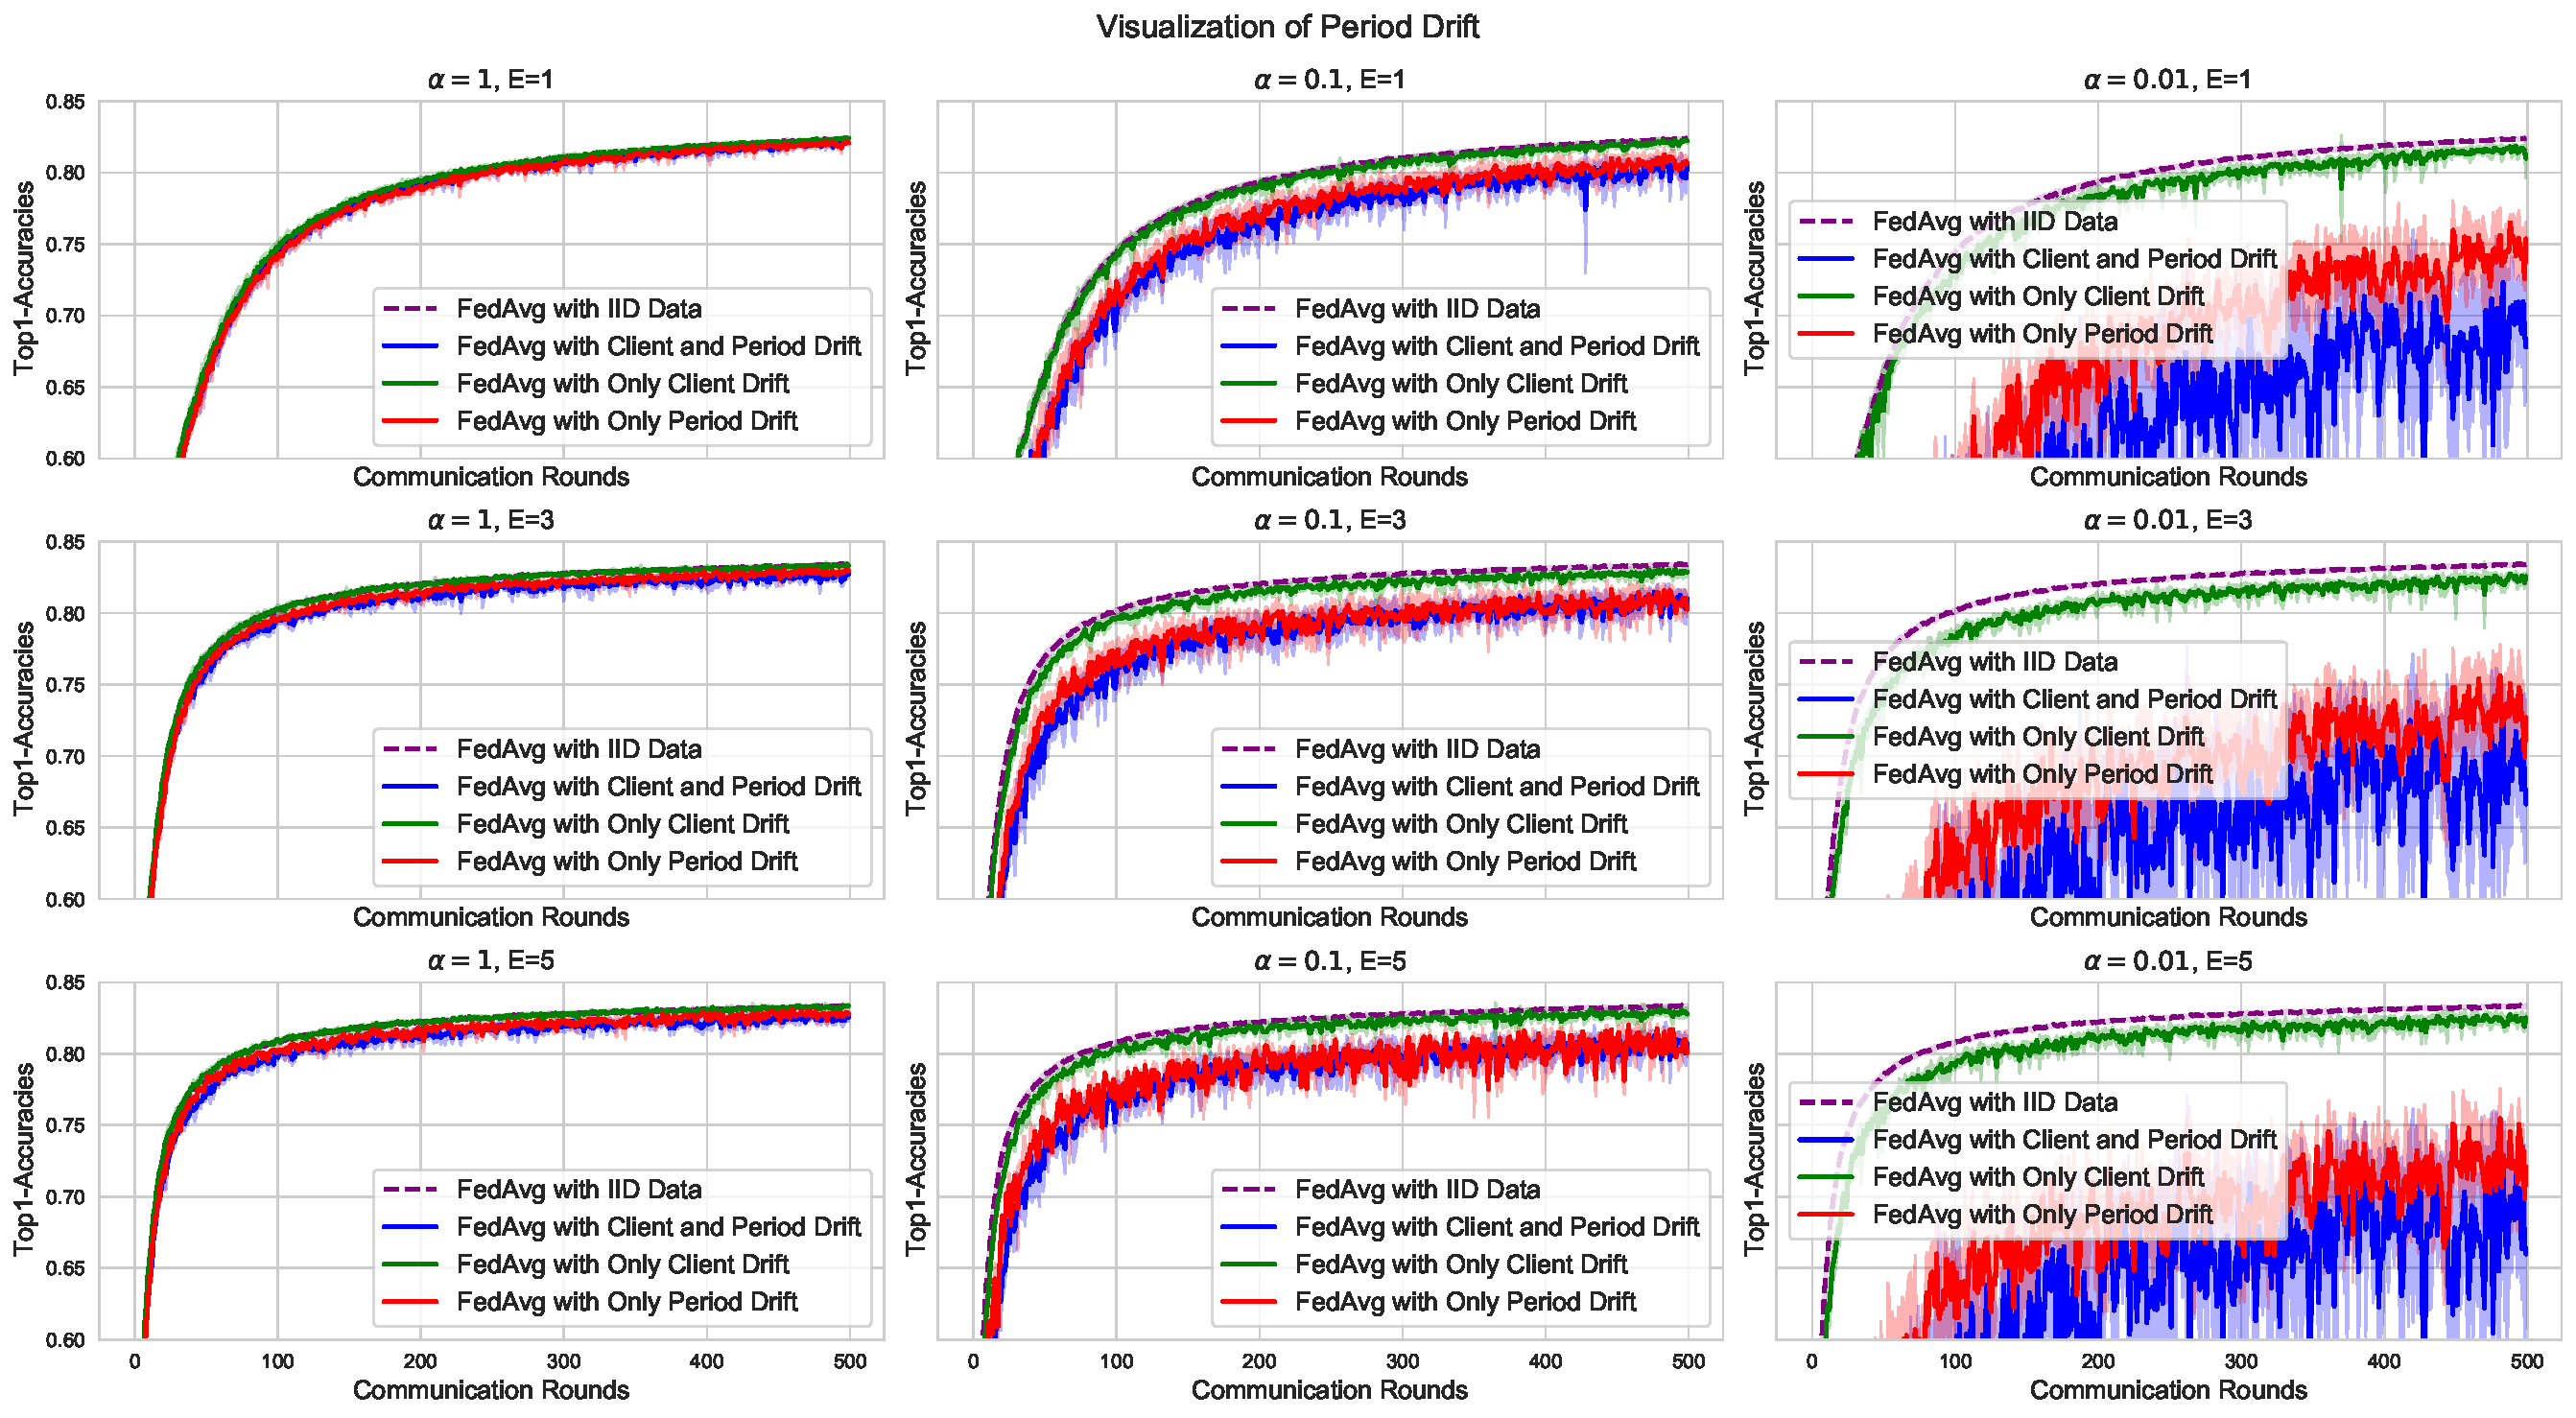
\includegraphics[width=0.65\linewidth]{visualization_of_period_drift.pdf}
    \caption{\small \textbf{Visualization of period drift with different $\alpha$ and $E$}}
\end{figure}
\begin{itemize}
    \item \textbf{Figure \ref{fig:visualize} (a).} To provide a clearer illustration, we displayed the label distribution of the 10-digit classes, rather than the complete 62 classes in the original FEMNIST dataset, for 20 communication rounds.
    \item \textbf{Figure \ref{fig:visualize} (b).}  1) \textit{\fedavg with iid data with no period or client drift:} \fedavg with iid data, where training data is randomly partitioned among all clients, resulting in no period or client drift; 2) \textit{\fedavg with only period drift:} non-iid data is initially partitioned, but the training data of the sampled clients is randomly reshuffled and iid-distributed evenly among clients in each round, resulting in period drift but no client drift; 3) \textit{\fedavg with only client drift:} iid data is initially partitioned, but the training data of the sampled clients in each round is re-partitioned in non-iid setting, resulting in client drift but no period drift; 4) \textit{\fedavg with both period and client drift:} \fedavg with non-iid data, where data is partitioned in non-iid setting, resulting in both period and client drift.
\end{itemize}
To make the results more convincing, we conducted more experiments on FEMNIST. Specifically, we add experiments with various local epochs and data heterogeneity. Each experiment is repeated 5 times, and the results are shown as follow:


% \subsection{Analysis of Kalman Gain in \fedeve.} 
% We conducted an in-depth analysis of the Kalman Gain $K$ of FedEve under various experimental 
% \begin{wrapfigure}{r}{0.5\linewidth}\label{fig:kalman_gain}
%   %\vspace{-4mm}
%   \includegraphics[width=\linewidth]{fedeve_Kalman.pdf}
%   %\vspace{-6mm}
%   \caption{\small\textbf{Boxplots for Kalman Factors}}
%   %\vspace{-5mm}
% \end{wrapfigure}
% % \begin{figure}[ht]
% %   \centering
% %   % %\vspace{-4mm}
% %   \includegraphics[width=\linewidth]{fedeve_Kalman.pdf}\label{fig:kalman_gain}
% %   %\vspace{-6mm}
% %   \caption{\small\textbf{Boxplots for Kalman Factors}}
% %   %\vspace{-5mm}
% %   \end{figure}
% settings, incorporating four levels. of data heterogeneity and various local epochs, as shown in Figure 4. We observed that as data heterogeneity increases (i.e., as the value of $\alpha$ decreases), the Kalman Gain $K$ progressively enlarges. With the rise of data heterogeneity, the period drift starts to play a more dominant role. In this context, the primary role of Kalman Gain $K$ is to adjust the weights between global and local updates, as depicted by Equation (\ref{step:pre_s}) and (\ref{step:G_{kal}}). Further, according to Equation (\ref{step:M}), the model update tends to trust local updates more, stabilizing the optimization process. For varied counts of local updates, the relative change in Kalman Gain $K$ is marginal. This is primarily because, in cross-device FL, the client drift is not a pivotal or dominant factor, which aligns with our prior analysis in Figure \ref{fig:visualize}.

 








